\chapter{Design Approach} \label{chap:designaproach}
%%%%%%Intoduction/description
Based on the requirements mentioned in Section \ref{sec:requirements} the approach shown in \autoref{fig:controllerDiagram} is designed. 
The system is designed to autonomously survey an area specified by some coordinates.

This is achieved by computing a path within the specified area, that preforms a sweeping motion with a predefined width.
The path is used as input into the controllers, making the vessel follow it. 
Additionally to improve the precision of the measurements the sensor data will be fused together before it's used as input for the controllers. 
%%%%% Path generation
begin{figure}[H]
    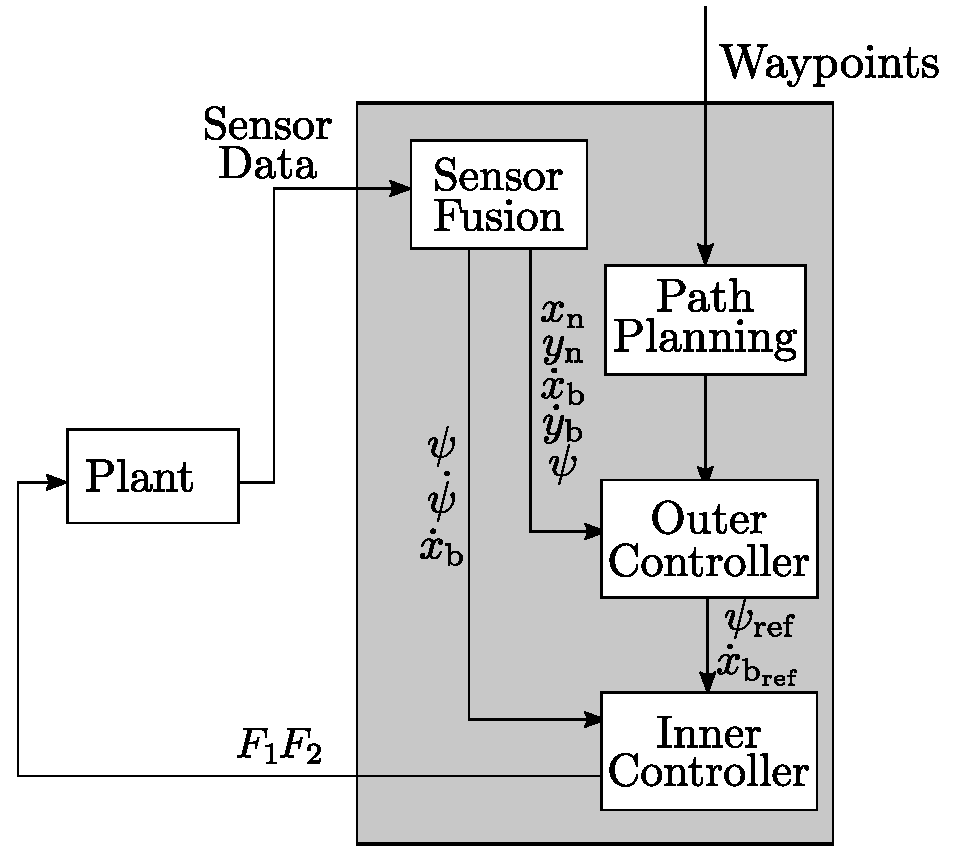
\includegraphics[width=0.3\textwidth]{figures/controllerDiagram2}
    \caption{}
    \label{fig:controllerDiagram}
\end{figure}

The control design consists of two controllers, an inner controller and an outer controller. 

As shown on \autoref{fig:controllerDiagram} the outer controller follows the path by changing the reference of the inner controller to obtain it's desired position. 
This approach is chosen as it separates the inertial frame from the boat frame, avoiding nonlinearities that would be present if a single controller used both frames of reference. 

The inner controller uses the references $\dot{x}_{bref}$ and $\dot{\psi}_{ref}$ to regulate $\dot{x}_{b}$ and $\dot{\psi}$ using $F_{1}$ and $F_{2}$. 
Two design approaches will be tested for the inner controller, an $H_{\infty}$ controller and a LQR controller.
The $H_{\infty}$ controller will be designed to be robust towards wind and wave disturbances and towards model errors. 
The LQR controller will be designed to reduce the energy consumption of the vessel and the states. 

The two approaches for the inner controller will be compared in the end, to see how each compares in the design categories; robustness and energy consumption. \fxnote{Make sure this is correct}

The outer controller is responsible for maintaining following a path in the inertial frame. 
The path received from the path generation algorithm represents a desired path for the boat to follow. \\

Using $x_{n}$ , $y_{n}$ $x_b$ $y_b$ and $\psi$ it is able to compute the $\psi_{ref}$ and $x_{ref}$ needed to follow the path. 

%%%%%Sensor Fusion%%%%%%
The sensor fusion is implemented to improve the precision of the measurements. 
The sensor fusion utilizes a kalmann filter to reduce measurement noise from the sensors, by comparing the measurements to a model of the vessel. 
The filter fuses the measured sensor data into $\psi$, $x_{b}$, $y_{b}$, $\dot{x}_{b}$ and $\dot{y}_{b}$ which is the states used by the controllers. 

